%% example.tex
%% Jeremy Singer
%% 16 Oct 12

\documentclass{mpaper}

\usepackage{tikz}
\usetikzlibrary{fit, arrows.meta}

\usepackage{siunitx}
\usepackage[basic]{complexity}
\usepackage[super,negative]{nth}
\usepackage[linesnumbered,lined,boxed,commentsnumbered]{algorithm2e}

\usepackage[labelfont=bf,textfont={bf,it}]{caption}
\usepackage{subcaption}
\usepackage{cleveref}

\usepackage{enumitem}
%\setlist{nosep}

\usepackage[backend=bibtex,maxnames=3,maxbibnames=99,style=trad-abbrv]{biblatex}
\addbibresource{mprop.bib}

% Addendum formatting (thanks, http://tex.stackexchange.com/questions/339471/indented-addendums-using-biblatex-sourcemaps)
% Also remove doi, url since unnecessary
\DeclareFieldFormat{addendum}{}
%\DeclareFieldFormat{url}{}
%\DeclareFieldFormat{doi}{}

\usepackage{xpatch}

\xpatchbibmacro{name:andothers}{%
	\bibstring{andothers}%
}{%
	\bibstring[\emph]{andothers}%
}{}{}

\definecolor{graphc1}{RGB}{150,227,240}
\definecolor{graphc2}{RGB}{250,71,37}
\definecolor{graphc3}{RGB}{253,161,77}
\definecolor{graphc4}{RGB}{141,246,135}

\begin{document}

\title{Graph Models and Maximum Common Subgraph for Character Analysis}
\author{Kyle A. Simpson}
\matricnum{2029567}

\maketitle
%====================================================
%====================================================
\begin{abstract}
%According to Simon Peyton Jones, an abstract should address
%four key questions. First, what is the problem that this
%paper tackles? Second, why is this an interesting problem?
%Third, what is the solution this paper proposes?
%Finally, why is the proposed solution a good one?
Lorem ipsum dolor sit amet lorem ipsum dolor sit amet lorem ipsum dolor sit amet lorem ipsum dolor sit amet lorem ipsum dolor sit amet lorem ipsum dolor sit amet lorem ipsum dolor sit amet lorem ipsum dolor sit amet lorem ipsum dolor sit amet lorem ipsum dolor sit amet lorem ipsum dolor sit amet lorem ipsum dolor sit amet lorem ipsum dolor sit amet lorem ipsum dolor sit amet lorem ipsum dolor sit amet lorem ipsum dolor sit amet lorem ipsum dolor sit amet lorem ipsum dolor sit amet lorem ipsum dolor sit amet lorem ipsum dolor sit amet lorem ipsum dolor sit amet

?? Write me
\end{abstract}
%====================================================
%====================================================

%====================================================
\section{Introduction}
\label{sec:introduction}
%====================================================

%?? Adapt proposal introduction
Research into computer vision tasks, such as image and object recognition, is currently dominated by the use of machine learning and vector-space models, while graph encodings are comparatively less well-explored.
%Neural networks and similar machine learning constructs learn features of the inputs and data they are given, which are later used to classify or identify patterns in images or generic datasets---and have become popular due to their versatility, effectiveness and accuracy across many problem domains.
Machine learning methods apply statistical inference from training data to teach classifiers how to recognise the desired elements or features from an image---and have become popular due to their versatility, effectiveness and accuracy across many problem domains.
Vector-space models, on the other hand, capture the area around high-contrast regions in images as salient features, or describe an image's contents in a dense and very low-level fashion.

In many cases it can be hard to reason about such models' robustness or sensitivity to different phenomena.
In a machine learning context, for instance, these are often a function of both the training data and the model itself.
The parameters learned by these models aren't structured in a way that allows humans to easily intuit what the model has learned or to comment on the system's correctness, and it can be difficult to discern \textit{why} a particular image might be misclassified.
Recent work into \emph{adversarial images} \cite{AdversarialML} has affirmed this, given that interference can lead to classifications contrary to image content.
%Outside of this, vector-space models can represent image interest points in a way that describes their neighbourhood (or indeed, the entirety of an image), and so are easier to understand; yet they lack any way to describe the relationships between these points or to capture an object's shape.

%?? Adversarial examples in ML \cite{AdversarialML}

Graph models, long-explored in discrete mathematics, provide a simpler way of visualising problems.
Systems are broken down into \emph{vertices} and \emph{edges} between vertex pairs---capturing the relationships between objects or key features within a scene.
For many domains, this is an intuitive and effective representation, encoding rich semantics in a very natural way which enjoys use in computational chemistry \cite{Graph-Molecules-2,Graph-Molecules-3,Graph-Molecules-1}, biology \cite{Graph-Biology-1}, and graph database analysis.
Furthermore, exact graph search and similarity metrics (e.g.\ the \emph{subgraph isomorphism} and \emph{maximum common subgraph} problems, respectively) are well-understood and an area of continual research in the field of algorithms.
%?? part of idea---need effective models to know that our similarity algorithms are a good fit?

The main aim of this paper is to explore the hypothesis that, after suitable transformation, image similarity corresponds to graph similarity according to these known metrics; \cref{fig:intro-sim} gives a rough illustration of the concept.
In particular, this work focuses on character analysis and recognition, considering both the performance of graph models within a domain alongside the usefulness of any chosen analytic techniques.
By investigating these questions, this paper contributes:
\begin{itemize}
	\item A demonstration of the shortcomings of existing image graph work for generic matching (\Cref{sec:image-weakness}), by attempting similarity computation on graphs built using common techniques from the literature. %given that this also requires an investigation into the effectiveness of known graph similarity techniques, this motivates the development of new models.
	This weakness motivates the development of new modelling strategies.
	\item ?? Detail as paper written
\end{itemize}

\begin{figure}
	\centering
	\resizebox{\columnwidth}{!}{
		\Large
		\begin{tikzpicture}
		\node[inner sep=5pt] (sagrada1) at (0,0)
		{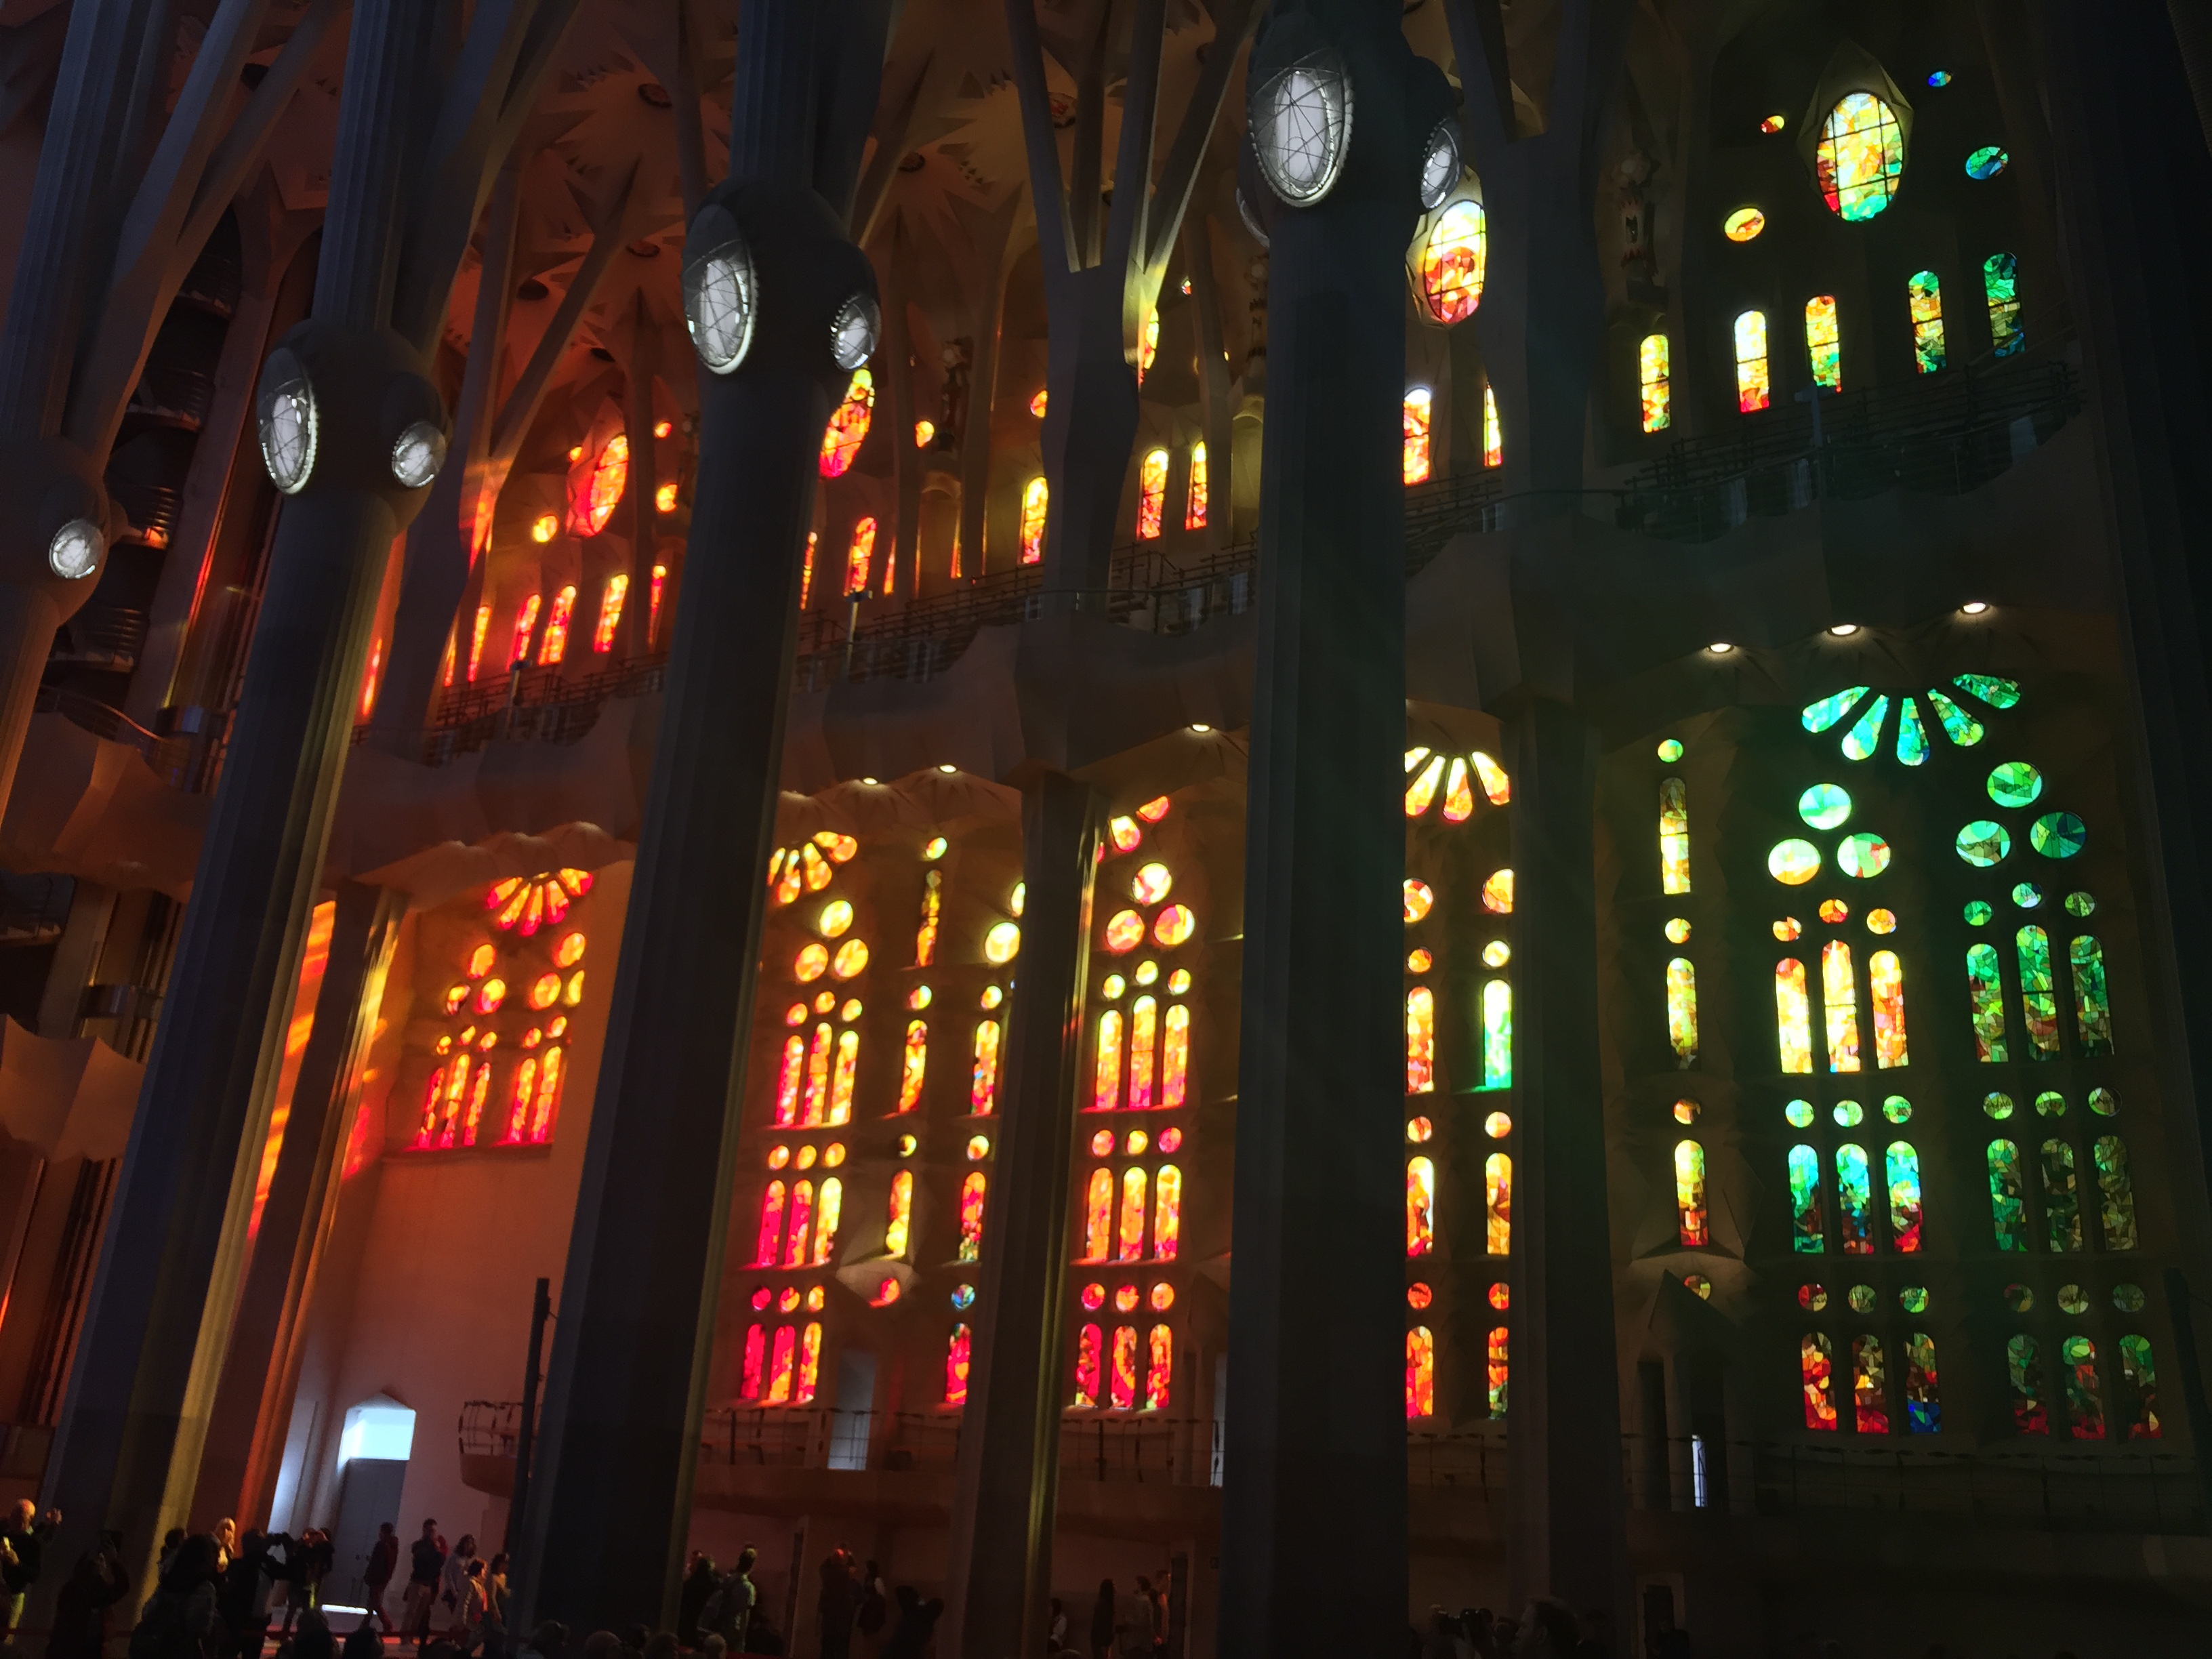
\includegraphics[width=.35\textwidth]{images/IMG_3267.JPG}};
		\node[inner sep=5pt] (sagrada2) at (10,0)
		{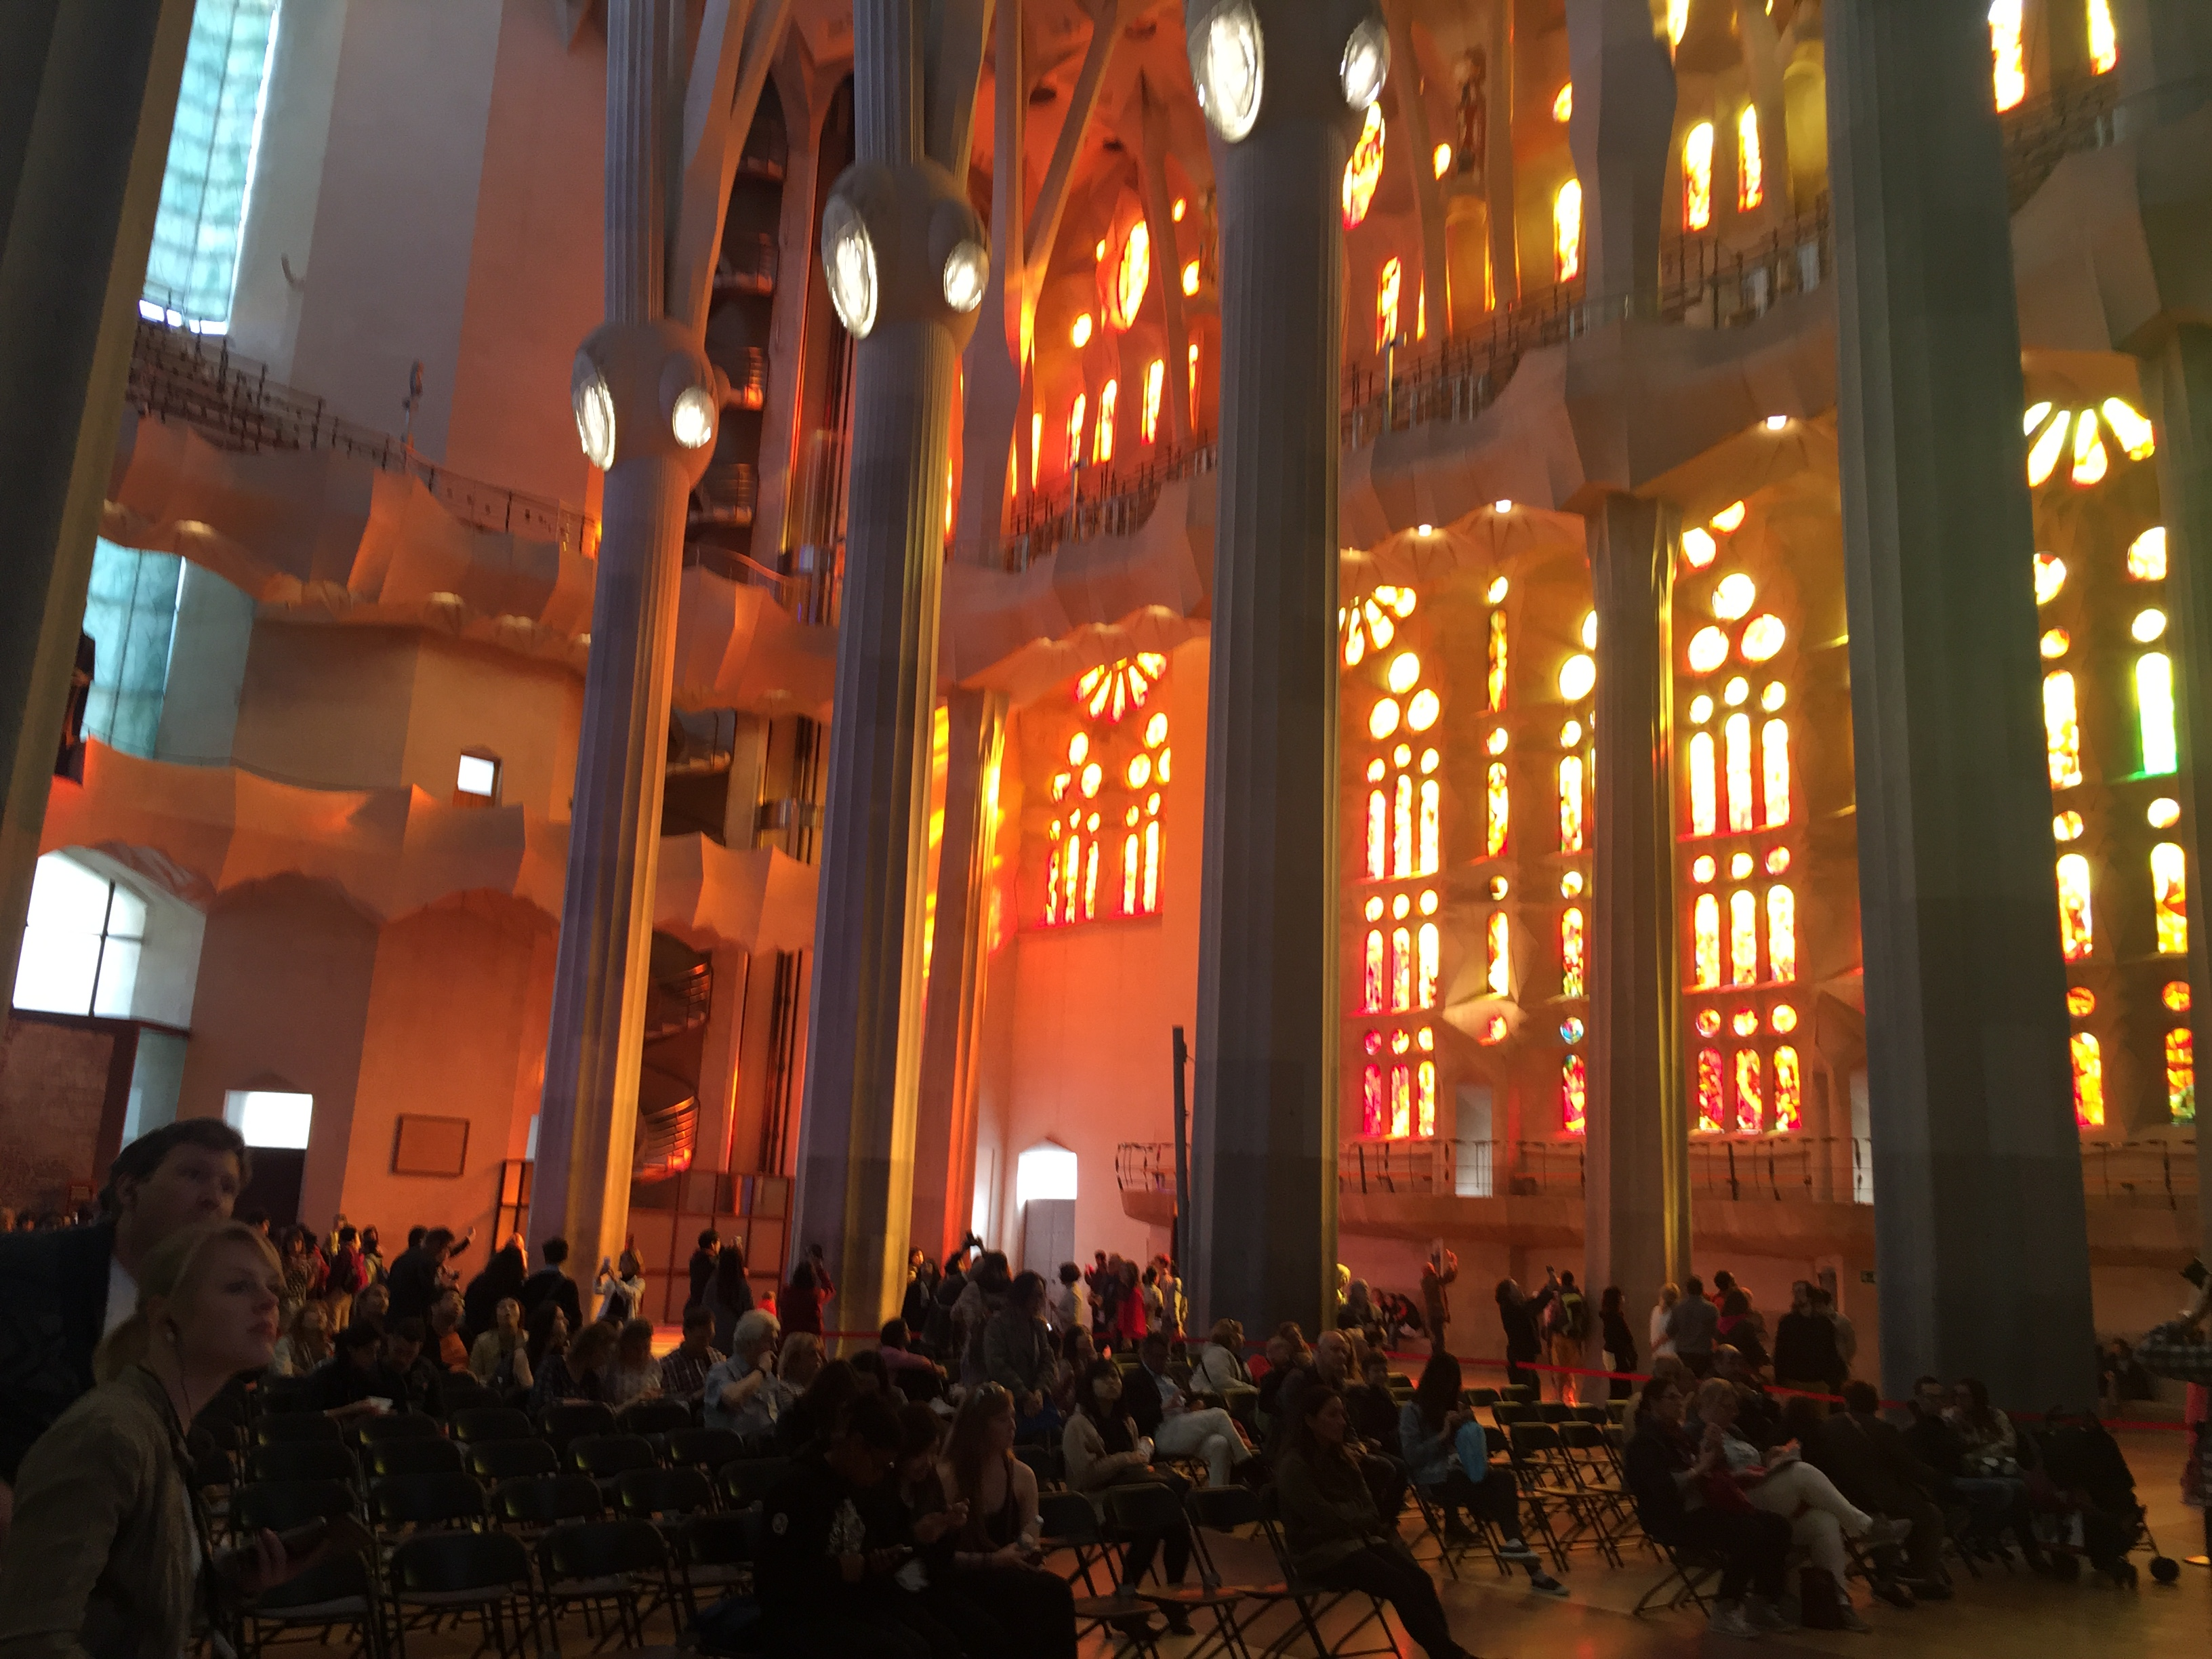
\includegraphics[width=.35\textwidth]{images/IMG_3268.JPG}};
		
		\node[inner sep=5pt] (graph1) at (0,-6)
		{
			\begin{tikzpicture}
			\node[draw, circle, fill=graphc2] (n1) at (0,-1) {};
			\node[draw, circle, fill=graphc3] (n2) at (1,-0.67) {};
			\node[draw, circle, fill=graphc4] (n3) at (2,-0.33) {};
			\node[draw, circle, fill=graphc2] (n4) at (0,-2) {};
			\node[draw, circle, fill=graphc3] (n5) at (1,-1.9) {};
			\node[draw, circle, fill=graphc4] (n6) at (2,-1.8) {};
			
			\draw[<->] (n1) -- (n2);
			\draw[<->] (n2) -- (n3);
			\draw[<->] (n1) -- (n4);
			\draw[<->] (n2) -- (n5);
			\draw[<->] (n4) -- (n5);
			\draw[<->] (n5) -- (n6);
			\end{tikzpicture}
		};
		
		\node[inner sep=5pt] (graph2) at (10,-6)
		{
			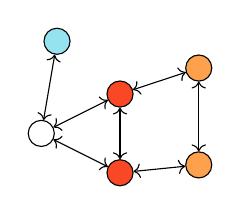
\begin{tikzpicture}
			\node[draw, circle] (n0) at (-1,-1.5) {};
			\node[draw, circle, fill=graphc1] (n7) at (-0.8,-0.33) {};
			\node[draw, circle, fill=graphc2] (n1) at (0,-1) {};
			\node[draw, circle, fill=graphc3] (n2) at (1,-0.67) {};
			\node[draw, circle, fill=graphc2] (n4) at (0,-2) {};
			\node[draw, circle, fill=graphc3] (n5) at (1,-1.9) {};
			
			\draw[<->] (n0) -- (n1);
			\draw[<->] (n0) -- (n4);
			\draw[<->] (n0) -- (n7);
			\draw[<->] (n1) -- (n2);
			\draw[<->] (n1) -- (n4);
			\draw[<->] (n2) -- (n5);
			\draw[<->] (n4) -- (n5);
			\end{tikzpicture}
		};
		
		\draw[->,thick] (sagrada1.east) -- (sagrada2.west)
		node[midway,fill=white] {Similarity};
		\draw[->,thick] (graph1.east) -- (graph2.west)
		node[midway,fill=white] {Similarity};
		
		\draw[->,thick] (sagrada1.south) -- (graph1.north)
		node[midway,fill=white] {Transform};
		\draw[->,thick] (sagrada2.south) -- (graph2.north)
		node[midway,fill=white] {Transform};
	\end{tikzpicture}
}
\caption{An example of the expected similarity between two views of the same scene. Similar objects and scenes should theoretically generate similar graphs after a suitable transformation, enabling recognition across images.\label{fig:intro-sim}}
\end{figure}

%====================================================
\section{Graphs, Search and Similarity}
\label{sec:graph-search}
%====================================================

%?? Graph definitions etc
First, we must define graphs more precisely.
An undirected graph $\mathcal{G}$ may be written $\mathcal{G} = (V,E)$ for a vertex set $V$ and an edge set $E \subseteq \lbrace \lbrace u,v \rbrace : u,v \in V \rbrace $, i.e.\ each edge $e \in E$ is a set of two nodes from $V$.
For some $u,v \in V$, we may write $u \sim_\mathcal{G} v$ to mean $u$ and $v$ are adjacent vertices in $\mathcal{G}$ ($\lbrace u,v \rbrace \in E$), and use $N_\mathcal{G}(u)$ to refer to $u$'s \emph{neighbourhood}---the set of all vertices in $V \backslash \lbrace u \rbrace$ adjacent to $u$ in $\mathcal{G}$.
This definition allows loops, e.g.\ $u \sim_\mathcal{G} u$ with the caveat that $u \notin N_\mathcal{G}(u)$.
Additionally, the \emph{order} of $\mathcal{G}$ refers to the count of $\mathcal{G}$'s vertices ($O(\mathcal{G})=|V|$), and the \emph{size} of $\mathcal{G}$ refers to the count of $\mathcal{G}$'s edges ($S(\mathcal{G})=|E|$).
Where $\mathcal{G}$ is clear from context, the relevant subscripts will be elided.

The graphs produced by the techniques I outline are \emph{attributed undirected multigraphs}: vertices and edges may have labels, and each pair of vertices may share multiple edges.
Given domains $L_v, L_e$ for vertex and edge labels respectively, we redefine $\mathcal{G} = (V,E,l_v,l_e)$ for a vertex set $V$, an edge set $E$, a vertex label mapping $l_v: V \rightarrow L_v$ and an edge mapping $l_e: E \rightarrow \lbrace(\lbrace u,v \rbrace, l): u,v \in V, l \in L_e\rbrace$.
%For any vertex $v \in V$, its label in $\mathcal{G}$ is given as $l_\mathcal{G}(v)$.
We can succinctly describe the edges between any $u, v \in V$ with a sorted (non-decreasing) sequence of labels, $seq_\mathcal{G}(u, v)$.
This allows us to define basic adjacency, and thus the basic neighbourhood: $u \sim_\mathcal{G} v \iff |seq_\mathcal{G}(u,v)| \ge 1$.
For matching such graphs, we require two new neighbourhood definitions.
Given a sorted label sequence $s$, we may define the \emph{exact neighbourhood} $N^{=}_{s,\mathcal{G}}(u)$ as the set of all $v \in N_\mathcal{G}(u)$ such that $seq_\mathcal{G}(u,v)=s$.
The \emph{sufficient neighbourhood} $N^{\succcurlyeq}_{s,\mathcal{G}}(u)$ is the set of all $v \in N_\mathcal{G}(u)$ where we may map each label in $s$ to a distinct label of equal value in $seq_\mathcal{G}(u,v)$---we say that $s \preccurlyeq seq_\mathcal{G}(u,v)$ if such a mapping exists.
%=\lbrace v \in V \backslash \lbrace u \rbrace: seq_\mathcal{G}(u,v)=s\rbrace$
For simplicity, I shall define the core search and similarity problems using undirected graphs.

Transformation from an image to a graph will create a graph whose structure corresponds to the image's content and invariants.
If an image $I$ contains an object, it is thus reasonable to assume that the graph produced from an image of only that object should be reproduced within $I$'s graph model---this may be useful when e.g., searching for a road sign in a view seen by an autonomous car.
This form of graph search is known as the \emph{subgraph isomorphism problem} (SIP), which is concerned with finding the exact structure of some pattern graph $\mathcal{P}=(V_\mathcal{P}, E_\mathcal{P})$ within a target graph $\mathcal{T}=(V_\mathcal{T}, E_\mathcal{T})$---an example is provided in \cref{fig:lit-sip}.
More precisely, for the non-induced variant of SIP the problem is to find an injective mapping $i : V_\mathcal{P} \rightarrow V_\mathcal{T}$ such that $\forall u,v \in V_\mathcal{P}, i(u) \neq i(v)$ and $u \sim_\mathcal{P} v \Rightarrow i(u) \sim_\mathcal{T} i(v)$, preserving adjacency and ensuring no two vertices of $\mathcal{P}$ are mapped to the same vertex of $\mathcal{T}$.
The induced variant additionally imposes that $\forall u,v \in V_\mathcal{P}, u \nsim_\mathcal{P} v \Rightarrow i(u) \nsim_\mathcal{T} i(v)$, ensuring that non-adjacent vertices in $\mathcal{P}$ must remain non-adjacent in the embedding in $\mathcal{T}$.
While SIP is \NP-Complete \cite{Cook-SAT-SIP-NP, Computers-and-Intractibility}, with modern algorithms such as \citeauthor{SIP-Glasgow}'s Glasgow solver it is computationally feasible for graphs on the order of several thousand vertices \cite{SIP-Glasgow}.
Trends in recent work have focused on increasing performance for larger instances through more costly filtering and pre-processing \cite{SIP-LAD, SIP-SND, SIP-Glasgow}---for this reason, older approaches such as VF2 \cite{SIP-VF2} remain competitive on smaller instances \cite{SIP-Hard-Instances}.
%The constraint programming 
%?? SIP \cite{SIP-VF2, SIP-LAD, SIP-SND, SIP-Glasgow}, Regin filtering \cite{AllDiff}, Complexity \cite{Cook-SAT-SIP-NP}

\begin{figure}
	\centering
	\resizebox{\columnwidth}{!}{
	\begin{tikzpicture}
	
	\node[label=below:{$\mathcal{P}$}] (p) at (0,0){
		\begin{tikzpicture}[scale=1]
		\node[draw, circle] (n1) at (0,0) {a};
		\node[draw, circle] (n2) at (0,-1) {c};
		\node[draw, circle] (n3) at (1,0) {b};
		\node[draw, circle] (n4) at (1,-1) {d};
		
		\draw[-] (n1) -- (n3);
		\draw[-] (n2) -- (n4);
		\draw[-] (n1) -- (n4);
		\draw[-] (n2) -- (n3);
		\draw[-] (n3) -- (n4);
		\end{tikzpicture}
	};
	
	\node[label=below:{$\mathcal{T}$}] (t) at (4,0){
		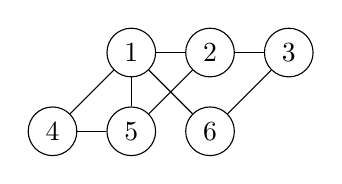
\begin{tikzpicture}[scale=1]
		\node[draw, circle] (n1) at (2,0) {2};
		\node[draw, circle] (n2) at (0,-1) {4};
		\node[draw, circle] (n3) at (1,0) {1};
		\node[draw, circle] (n4) at (1,-1) {5};
		
		\node[draw, circle] (n5) at (2,-1) {6};
		\node[draw, circle] (n6) at (3,0) {3};
		
		\draw[-] (n1) -- (n3);
		\draw[-] (n2) -- (n4);
		\draw[-] (n1) -- (n4);
		\draw[-] (n2) -- (n3);
		\draw[-] (n3) -- (n4);
		
		\draw[-] (n5) -- (n6);
		\draw[-] (n1) -- (n6);
		\draw[-] (n3) -- (n5);
		\end{tikzpicture}
	};
	
	\node[label=below:{Embedding}] (em) at (9,0){
		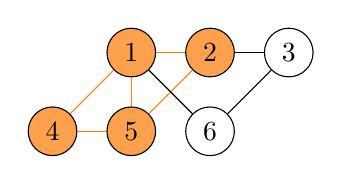
\begin{tikzpicture}[scale=1]
		\node[draw, circle, fill=graphc3] (n1) at (2,0) {2};
		\node[draw, circle, fill=graphc3] (n2) at (0,-1) {4};
		\node[draw, circle, fill=graphc3] (n3) at (1,0) {1};
		\node[draw, circle, fill=graphc3] (n4) at (1,-1) {5};
		
		\node[draw, circle] (n5) at (2,-1) {6};
		\node[draw, circle] (n6) at (3,0) {3};
		
		\draw[-, color=orange] (n1) -- (n3);
		\draw[-, color=orange] (n2) -- (n4);
		\draw[-, color=orange] (n1) -- (n4);
		\draw[-, color=orange] (n2) -- (n3);
		\draw[-, color=orange] (n3) -- (n4);
		
		\draw[-] (n5) -- (n6);
		\draw[-] (n1) -- (n6);
		\draw[-] (n3) -- (n5);
		\end{tikzpicture}
	};
	
	\draw[->, thick] (t) -- (em);
	
\end{tikzpicture}
}
\caption{
		An example of the subgraph isomorphism problem between two graphs $\mathcal{P}$ and $\mathcal{T}$.
		$\mathcal{P}$'s embedding within $\mathcal{T}$ is highlighted in orange---this is a valid matching in both the induced and non-induced SIP variants.
		\label{fig:lit-sip}
}
\end{figure}

%?? MCS \cite{Between-MCS-SIP}, James+Ciaran+Pat's new paper too \cite{MCS-McSplit}, complexity \cite[p.\ 74--75]{Computers-and-Intractibility}
In reality, elements of an object's graph structure may not be reproduced in the graph of an embedding due to either occlusion, image distortion or object scale.
In this case, it is worthwhile to examine how much two image graphs have in common to identify common elements and substructures.
Between two graphs $\mathcal{P}$ and $\mathcal{T}$ this is known as the \emph{maximum common subgraph problem} (MCS), which is the search for the largest subgraph of $\mathcal{P}$ which is isomorphic to some subgraph of $\mathcal{T}$ as in SIP.
\Cref{fig:lit-mcs} offers an example instance.
While this problem is also \NP-Complete \cite[p.\ 74--75]{Computers-and-Intractibility}, it is considerably harder in practice than SIP---the current state-of-the-art, McSplit, can operate on graphs of order 35--40 \cite{MCS-McSplit}, where other approaches are limited to around 30 vertices.
Even so, this approach applies only to the induced variant of MCS and largely prevents the addition of side constraints.
For such flexibility we must consider either $k\downarrow$ \cite{Between-MCS-SIP}, a repeated application of the Glasgow SIP solver excluding $k$ vertices, or a max-clique-based approach using the \emph{association graph encoding} \cite{MCS-Clique-CP}.
In this regard there is a trade-off to be made: while the clique-based approach still achieves the best performance on labelled instances \cite{MCS-McSplit}, $k\downarrow$ requires far less memory to process high-order graphs.
I choose to examine and modify $k\downarrow$ for these reasons, but this still requires that the order of any graphs must remain small to perform occlusion-robust matching with this technique.

By computing similar structures between any two graphs as above, we may then quantify how similar they are by considering the order of the MCS.
This is in turn a key part of establishing how \emph{dissimilar} a pair of graphs are, and given that MCS order does not take into account the sizes of $\mathcal{P}$ or $\mathcal{T}$ such a metric is more desirable for global classification.
We may then use the MCS to compute the number of discrete changes needed to transform $\mathcal{P}$ into $\mathcal{T}$---the \emph{graph edit distance} (GED) \cite{GraphEditDist-MCS}.
For classification purposes, I consider a simplified expression which disregards edge costs:
$$ GED(\mathcal{P}, \mathcal{T}) = O(\mathcal{P}) + O(\mathcal{T}) - 2 O(MCS(\mathcal{P}, \mathcal{T})) $$

\begin{figure}
	\centering
	\resizebox{\columnwidth}{!}{
	\begin{tikzpicture}
	
	\node[label=below:{$\mathcal{P}$}] (p) at (0,0){
		\begin{tikzpicture}[scale=1]
		\node[draw, circle] (n1) at (0,0) {a};
		\node[draw, circle] (n2) at (0,-1) {c};
		\node[draw, circle] (n3) at (1,0) {b};
		\node[draw, circle] (n4) at (1,-1) {d};
		
		\draw[-] (n1) -- (n3);
		\draw[-] (n2) -- (n4);
		\draw[-] (n1) -- (n4);
		\draw[-] (n2) -- (n3);
		\draw[-] (n3) -- (n4);
		\end{tikzpicture}
	};
	
	\node[label=below:{$\mathcal{T}$}] (t) at (3,0){
		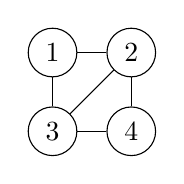
\begin{tikzpicture}[scale=1]
		\node[draw, circle] (n1) at (0,0) {1};
		\node[draw, circle] (n2) at (0,-1) {3};
		\node[draw, circle] (n3) at (1,0) {2};
		\node[draw, circle] (n4) at (1,-1) {4};
		
		
		\draw[-] (n1) -- (n3);
		\draw[-] (n2) -- (n4);
		\draw[-] (n1) -- (n2);
		\draw[-] (n2) -- (n3);
		\draw[-] (n3) -- (n4);
		
		\end{tikzpicture}
	};
	
	\node[label=below:{Embedding}] (em) at (7,0){
		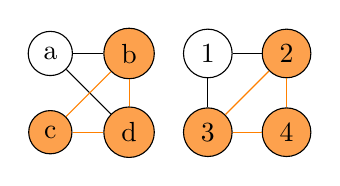
\begin{tikzpicture}[scale=1]
		\node[draw, circle] (n1) at (0,0) {a};
		\node[draw, circle, fill=graphc3] (n2) at (0,-1) {c};
		\node[draw, circle, fill=graphc3] (n3) at (1,0) {b};
		\node[draw, circle, fill=graphc3] (n4) at (1,-1) {d};
		
		\draw[-] (n1) -- (n3);
		\draw[-, color=orange] (n2) -- (n4);
		\draw[-] (n1) -- (n4);
		\draw[-, color=orange] (n2) -- (n3);
		\draw[-, color=orange] (n3) -- (n4);
		
		\node[draw, circle] (n1') at (2,0) {1};
		\node[draw, circle, fill=graphc3] (n2') at (2,-1) {3};
		\node[draw, circle, fill=graphc3] (n3') at (3,0) {2};
		\node[draw, circle, fill=graphc3] (n4') at (3,-1) {4};
		
		
		\draw[-] (n1') -- (n3');
		\draw[-, color=orange] (n2') -- (n4');
		\draw[-] (n1') -- (n2');
		\draw[-, color=orange] (n2') -- (n3');
		\draw[-, color=orange] (n3') -- (n4');
		
		\end{tikzpicture}
	};
	
	\draw[->, thick] (t) -- (em);
	
\end{tikzpicture}
}
\caption{
		An example of the maximum common subgraph problem between two graphs $\mathcal{P}$ and $\mathcal{T}$.
		The MCS's embedding within both $\mathcal{P}$ and $\mathcal{T}$ is highlighted in orange.
		Note that this embedding is not unique, although for this choice of $\mathcal{P}$ and $\mathcal{T}$ the MCS itself is.
		\label{fig:lit-mcs}
}
\end{figure}

%====================================================
\section{On Existing Image Graph Models}
\label{sec:image-weakness}
%====================================================

%\citeauthor{Plane-Graphs-From-Images} \cite{Plane-Graphs-From-Images}

%?? Approaches such as seen in \cite{Submap-Iso-Images} use Delaunay -- Enhanced by structural cues such as in \cite{Plane-Graphs-From-Images}

\begin{figure*}
	\centering
	\begin{subfigure}[b]{0.22\textwidth}
		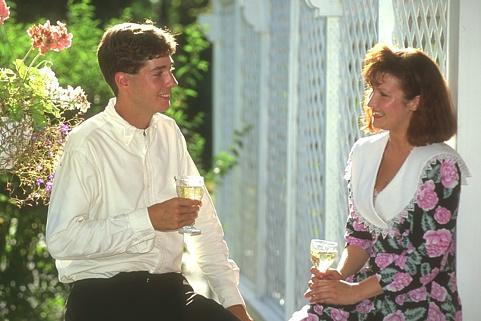
\includegraphics[width=\textwidth]{images/bsd-157055}
		\caption{BSD test image}
		\label{fig:explor-bsd}
	\end{subfigure}
	~
	\begin{subfigure}[b]{0.35\textwidth}
		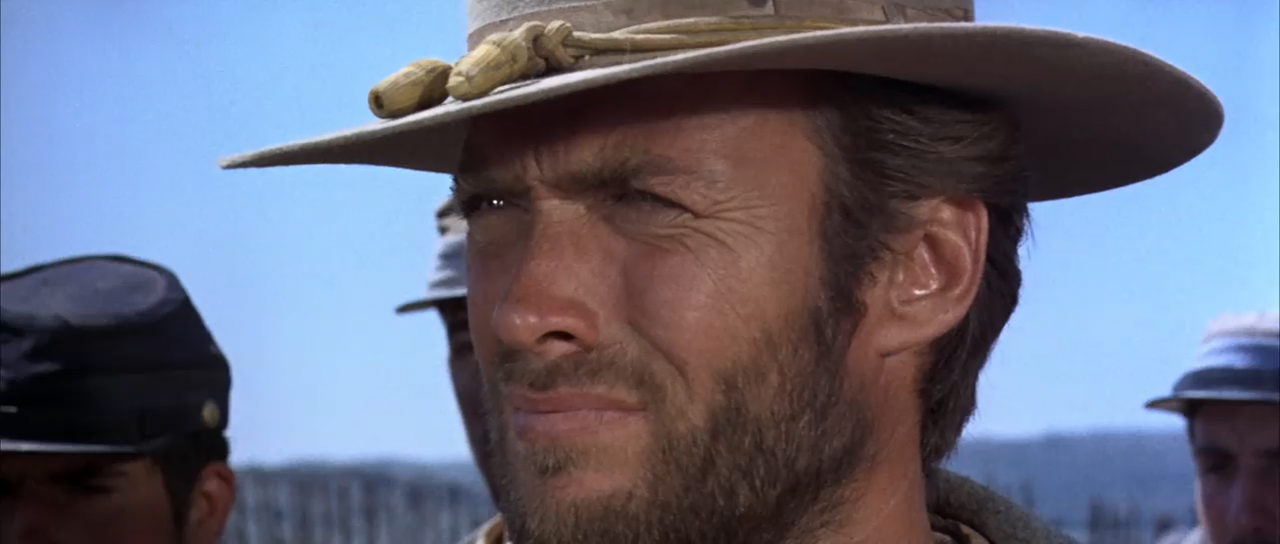
\includegraphics[width=\textwidth]{images/gbu2}
		\caption{Film frame 1}
		\label{fig:explor-ff1}
	\end{subfigure}
	~
	\begin{subfigure}[b]{0.35\textwidth}
		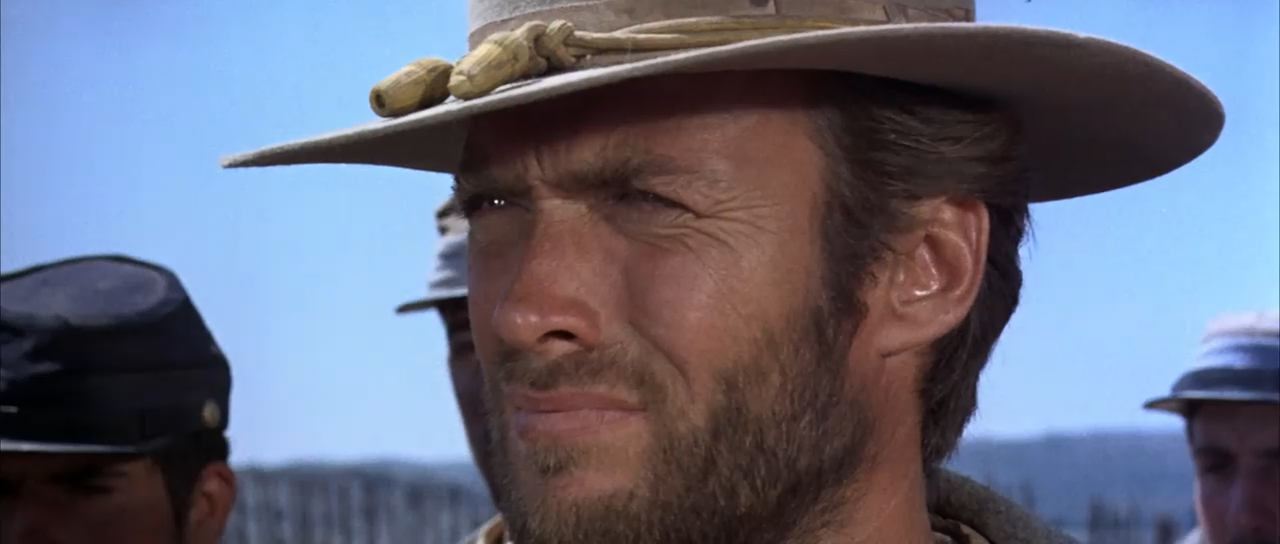
\includegraphics[width=\textwidth]{images/gbu3}
		\caption{Film frame 2}
		\label{fig:explor-ff2}
	\end{subfigure}
	
	\vspace{0.5em}
	
	\caption{
		Images used for evaluation of \citeauthor{Plane-Graphs-From-Images}'s \cite{Plane-Graphs-From-Images} approach.
	}
\end{figure*}

\begin{figure*}
	\centering
	\begin{subfigure}[b]{0.22\textwidth}
		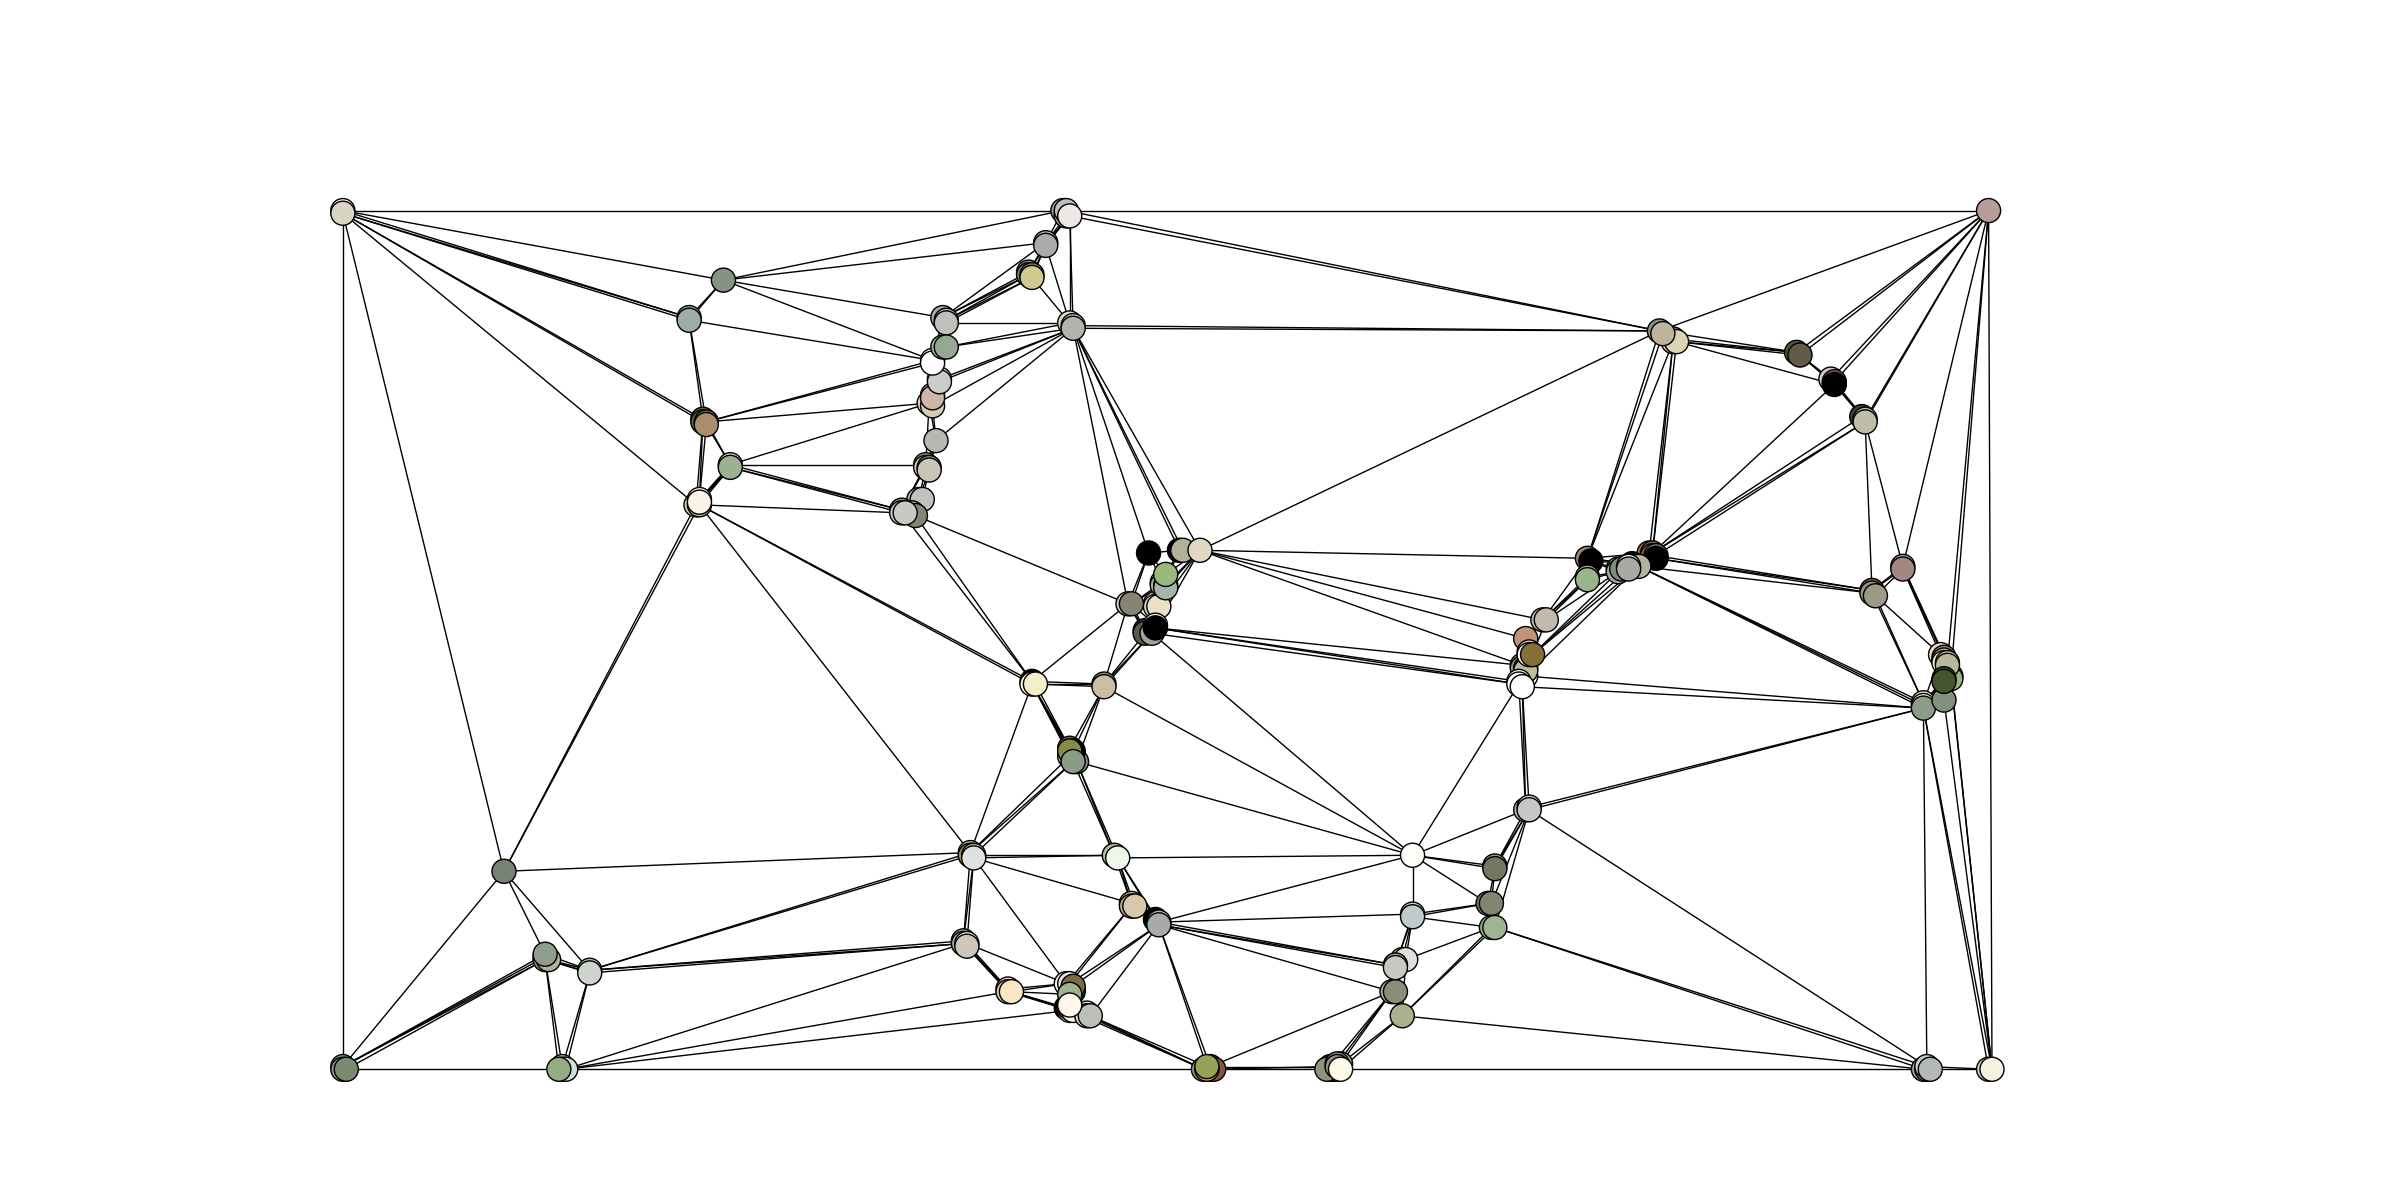
\includegraphics[width=\textwidth]{img-results/nrm}
		\caption{
				BSD test image, normal.
				$|V|=245$, $|E|=707$.
		}
		\label{fig:explor-bsdnrmgraph}
	\end{subfigure}
	~
	\begin{subfigure}[b]{0.22\textwidth}
		
\includegraphics[width=\textwidth]{img-results/180}
		\caption{
				BSD test image, \SI{180}{\degree} rotation.
				$|V|=247$, $|E|=705$.
		}
		\label{fig:explor-bsd180graph}
	\end{subfigure}
	~
	\begin{subfigure}[b]{0.22\textwidth}
		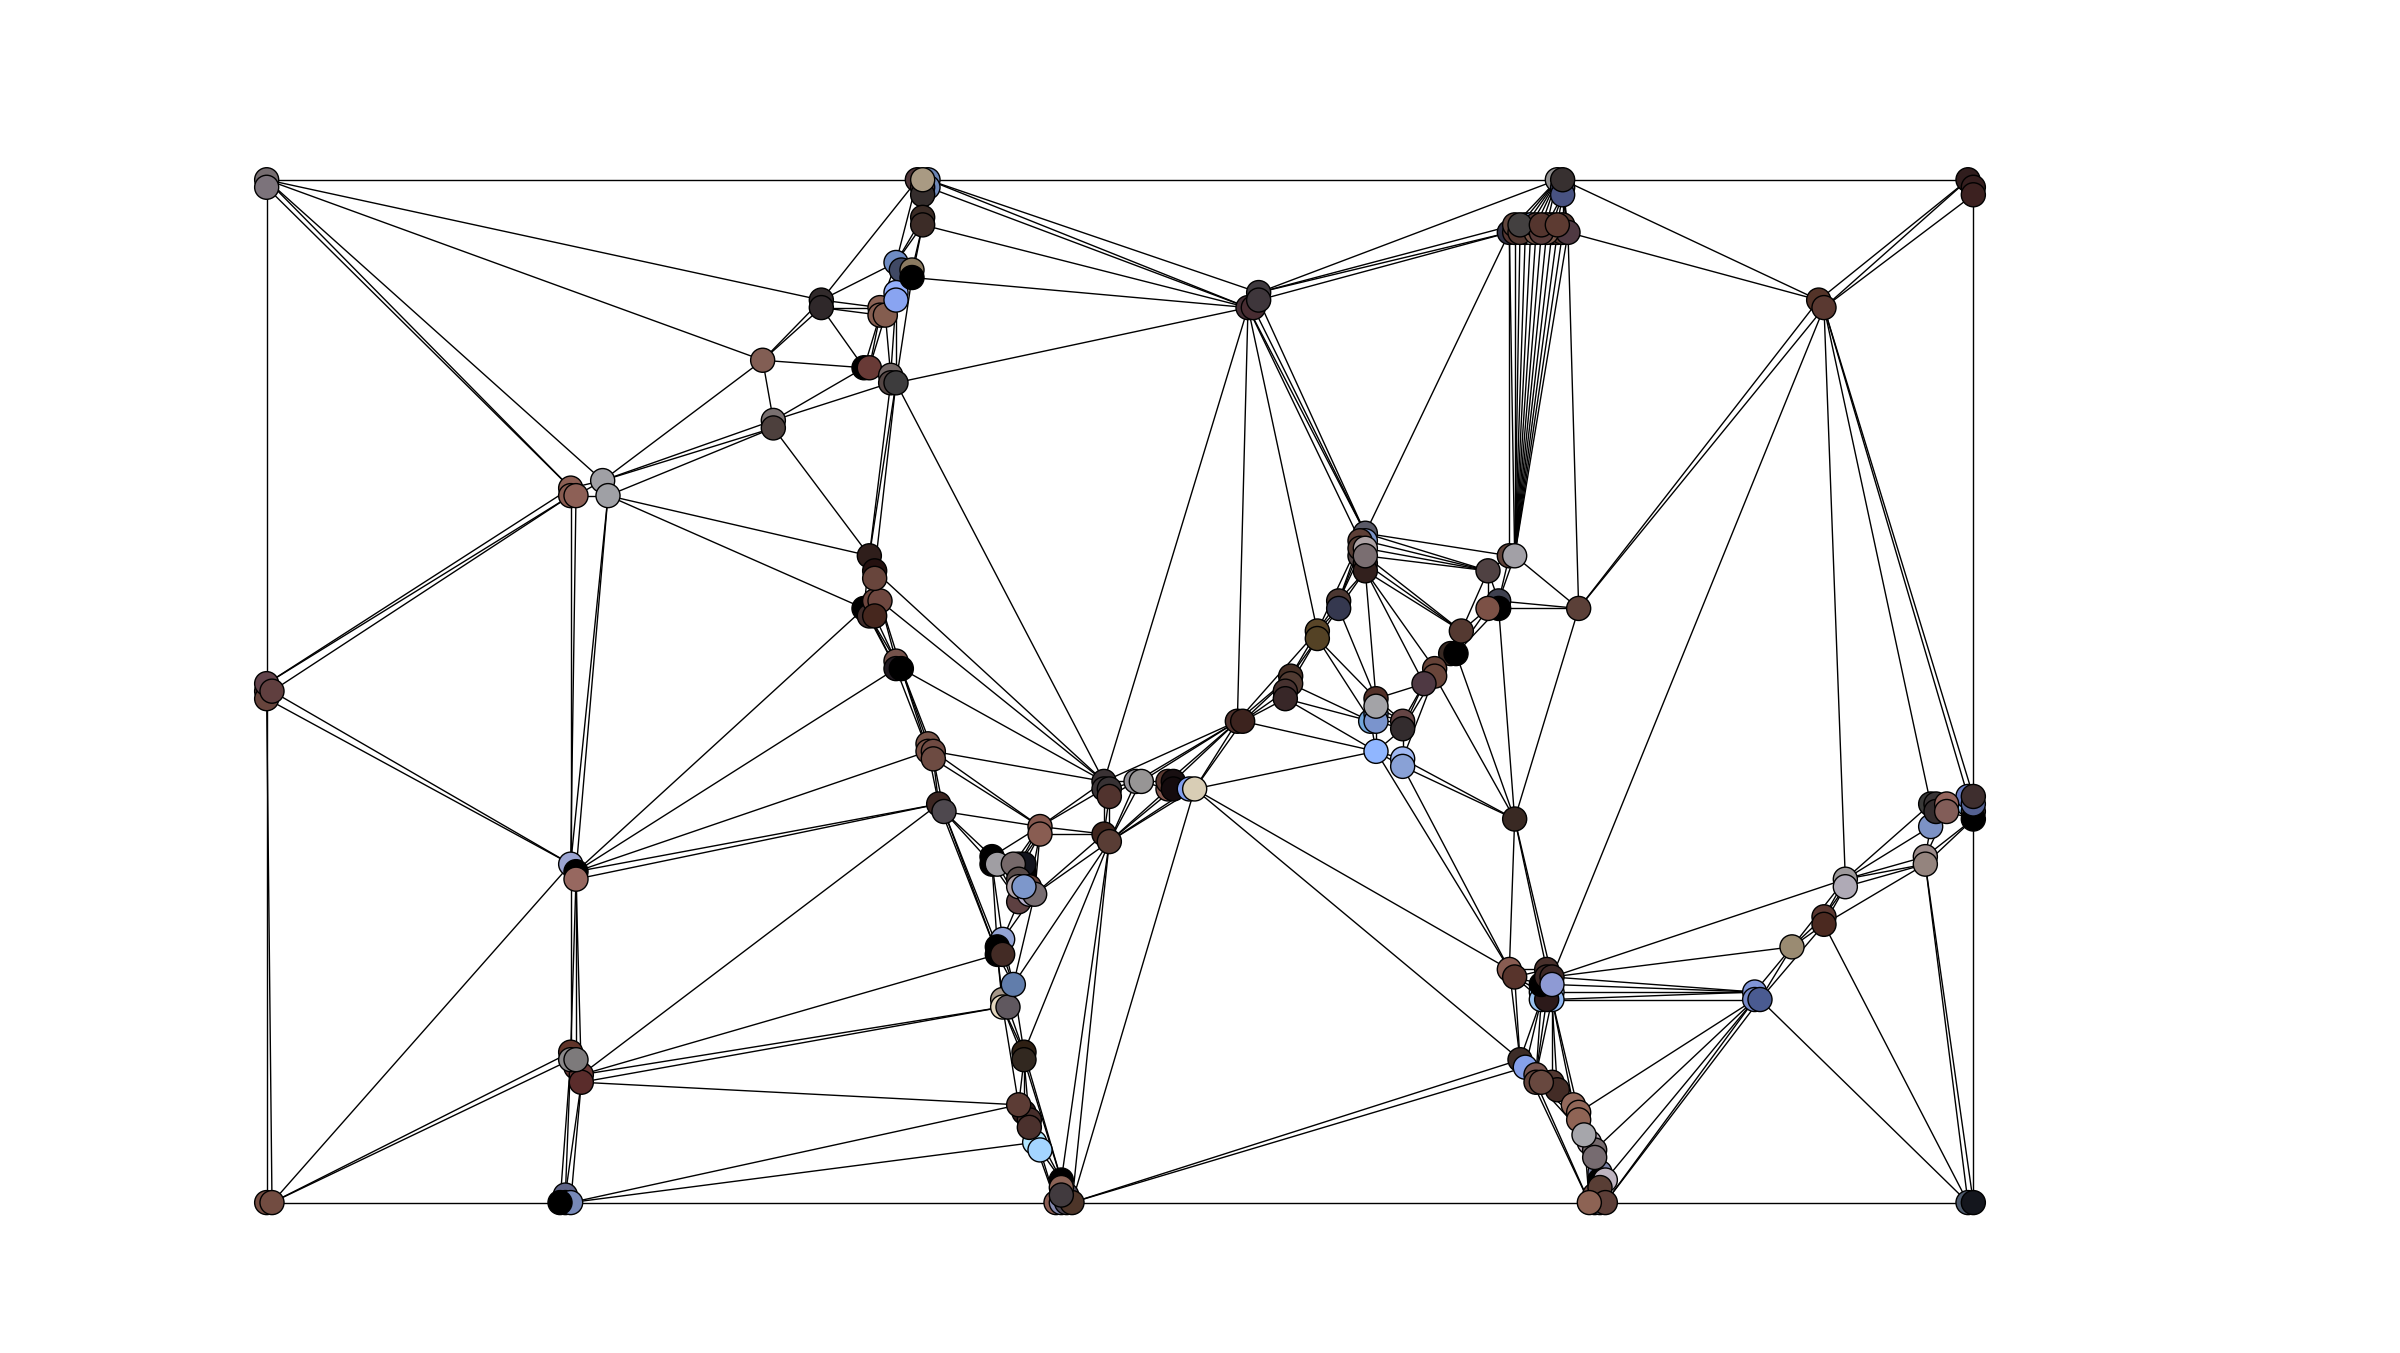
\includegraphics[width=\textwidth]{img-results/gbu-smr2-graph}
		\caption{
				Film frame 1.
				$|V|=264$, $|E|=755$.
		}
		\label{fig:explor-ff1graph}
	\end{subfigure}
	~
	\begin{subfigure}[b]{0.22\textwidth}
		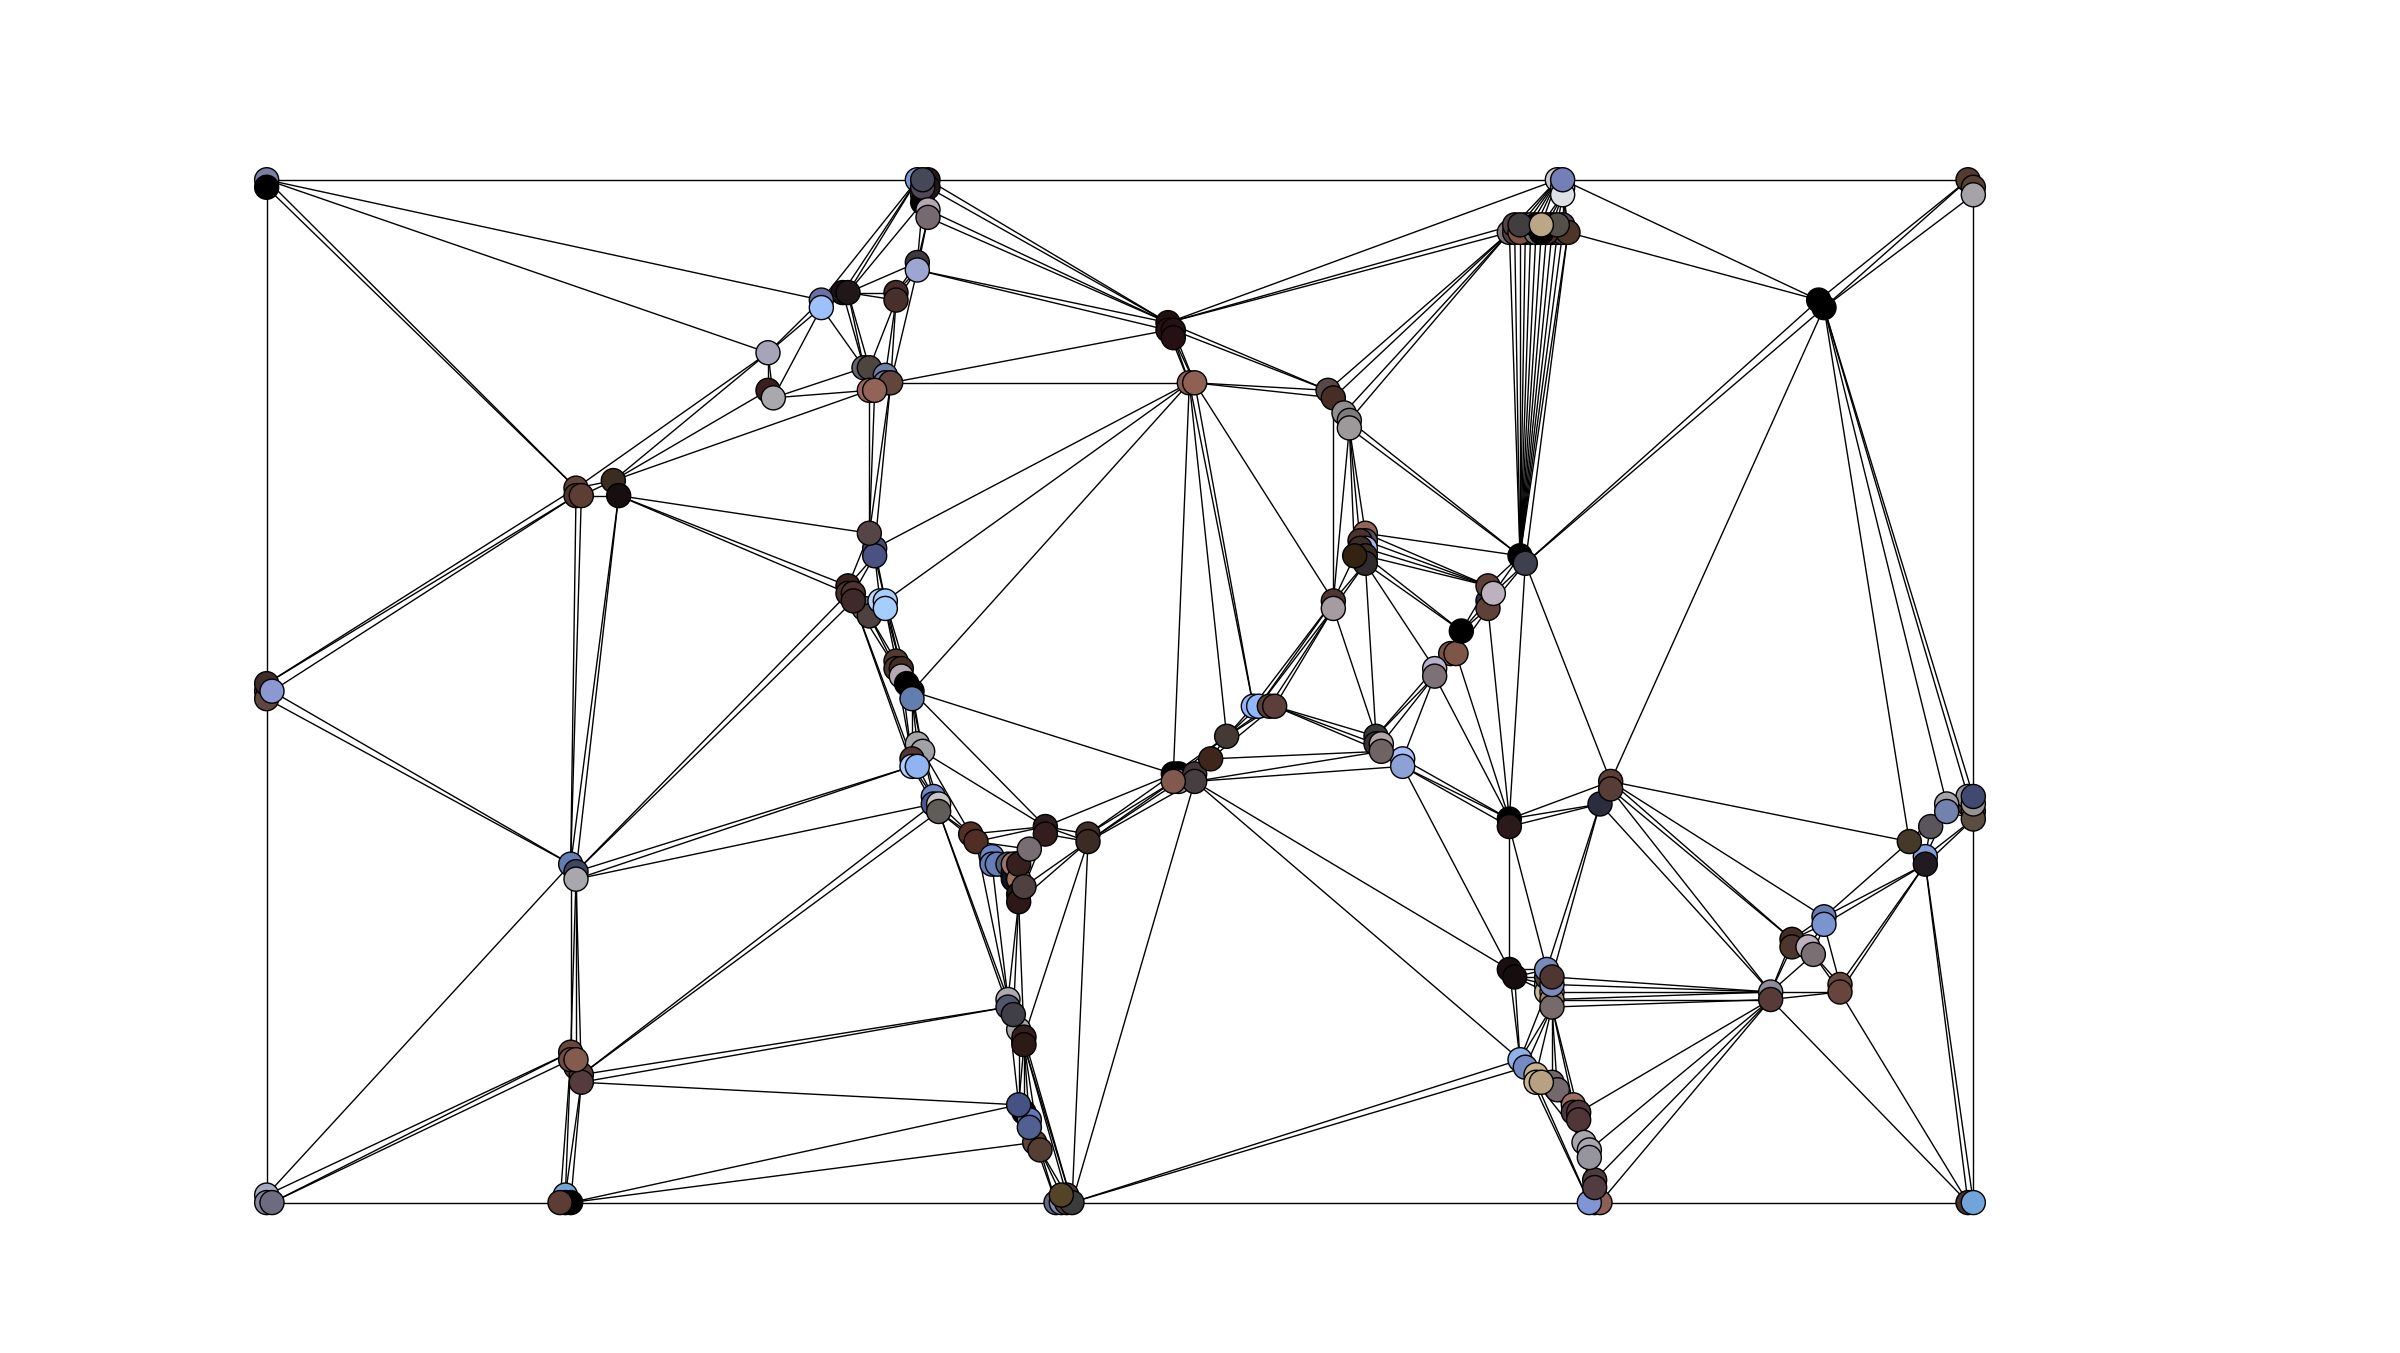
\includegraphics[width=\textwidth]{img-results/gbu-smr3-graph}
		\caption{
				Film frame 2.
				$|V|=260$, $|E|=743$.
		}
		\label{fig:explor-ff2graph}
	\end{subfigure}
	
	\vspace{0.5em}
	
	\caption{
		Graph output after boundary walking and Delaunay triangulation.
		$|V|$ and $|E|$ denote the vertex count and edge count, respectively.
	}
\end{figure*}

For graph modelling of generic images, present techniques typically build graphs by applying the Delaunay triangulation to a set of interest pixels located within an image.
This is explored briefly by \citeauthor{Submap-Iso-Images} \cite{Submap-Iso-Images}, and expanded upon by \citeauthor{Plane-Graphs-From-Images} to make use of structural cues provided by image segmentation algorithms \cite{Plane-Graphs-From-Images}.
The authors of these approaches assess the effectiveness of their models by either searching for an image cropping within itself (using \emph{submap} isomorphism) or by quantifying the ``loss'' incurred by reconstruction from the generated graph.
In this regard much is made of matching of graphs \emph{within} an image, and not \emph{between} images; making it unclear whether any discriminative features are captured or modelled in a way that allows matching using MCS algorithms.

%?? Use existing work from proposal as basis
%?? No capture of discriminative features
To investigate this, I implemented \citeauthor{Plane-Graphs-From-Images}'s algorithm in Python, using \textit{scikit-image}\footnote{\url{http://scikit-image.org/}} functions for segmentation and interest pixel detection.
Two experiments were performed:
\begin{enumerate}
	\item Establishing whether graphs of a test image from the Berkeley Segmentation Dataset \cite{BerkeleyDatabase} (\cref{fig:explor-bsd}) before and after \SI{180}{\degree} rotation were isomorphic, and measuring their similarity if not.
	\item Measuring the similarity between two adjacent frames of Sergio Leone's \emph{The Good, the Bad and the Ugly} (\cref{fig:explor-ff1} and \subref{fig:explor-ff2}).
\end{enumerate}
As the image graphs were expected to be high-order, nodes were labelled with their $(x,y)$ image locations to augment the $k\downarrow$ procedure with Euclidean distance filtering to make matching feasible---nodes could be mapped to one another if their distance was smaller than 1 for the first, or 5 for the second experiment.
These distances were chosen due to the expected similarity in each case---while the first experiment governs essentially identical images (once positions have been corrected to negate the transform), in the second case mild variance is expected.

\Cref{fig:explor-bsdnrmgraph,fig:explor-bsd180graph} show that the expected isomorphism in the first experiment was \emph{not} observed---both graphs have different order and size.
After 5 days runtime, the graph order was not exactly identified in either case, but the following bounds were obtained:

\begin{table}[h]
\centering
\begin{tabular}{|c|c|c|c|}
	\hline
	Experiment & Except-$k$ & $O(MCS)$ & Overlap (\si{\percent}) \\ \hline
	1 & $[61, 111]$ & $[134, 184]$ & 54.6--72.2 \\
	2 & $[38, 217]$ & $[47, 226]$ & 18.1--86.9 \\
	\hline
\end{tabular}
\end{table}

\noindent Due to the difficulty of finding an exactly optimal $k$, both of these results have an unacceptably high degree of uncertainty---we cannot draw any conclusive answers on the actual graph similarity for this reason.
The level of uncertainty here is strongly tied to the level of filtering provided in each experiment: a higher distance threshold gives more candidate mappings for each node, and so weaker filtering.
The bound in the first experiment is, however, low enough for two identical images to assert that this transformation is not isotropic.
This heavily indicates that the approach's validity and sensitivities depend upon the choice of interest pixel detector.
Furthermore, the presence of more unique structures would improve matching performance---I believe that the structure offered by the Delaunay triangulation is too uniform, and thus hinders our ability to compute the MCS.
Aside from this, the reliance on perfect segmentation (which is available within the Berkeley Segmentation Dataset) is clear---the second experiment required significant manual parameter tuning to acquire a reasonable segmentation, despite the exceptionally clear foreground-background distinction.
Most pressingly, this shows that the current work is wholly inappropriate for the task of image matching with currently available tools: extremely high-order graphs with little discriminative structure are produced, making analysis computationally infeasible.

%====================================================
\section{The Algorithm}
\label{sec:algorithm}
%====================================================

?? Graph gen algo -- kinda explain this guy's path splitting algo \cite{PathCurvature}

?? High-level diagram, walkthrough (like the example in the proposal)

?? Give example of (and explain) Z, H, K isomorphism in this scheme

?? introduce the ``dual'' representation (frame it like ``the graph models allowed me to learn \emph{why} these characters weren't distinct, and modify the algorithm to include path angle dynamics'')

%====================================================
\section{Modifications to k-Down}
\label{sec:k-down-mods}
%====================================================

?? Discuss/introduce $s$-adjacency (Already added $N^{=}_{s},N^{\succcurlyeq}_{s}$ to graph definitions section), and 3 levels of filtering (induced, edge-count-increasing, barely overlapping)

?? Keep standard filtering from supplemental graphs (adjacency matrix operates on at least 1-adjacency, exact matches are provided)

?? Could use path-based inference for new supplemental graphs, but probably way too much work for graphs of this order (i.e.\ very small)

?? Filtering at top of search---modify loop constraints, node label matching

?? Per-node of search, look at $s$-neighbourhoods

%====================================================
\section{Empirical Evaluation and Discussion}
\label{sec:evaluation}
%====================================================

?? Machine statistics, find the code here\footnote{\url{https://github.com/FelixMcFelix/sip-for-cv-paper}}, roll up a nice VM for review?

?? Heatmaps per font -- examine size? font v font? sans vs serif? Dual vs regular? How do the different filtering levels affect character distinctness?

?? Matching effectiveness statistics with HWRT \cite{HwrtDatabase} (Discuss effects of pen thickness, filtering class, dual vs regular). kNN classifier ($k=5$ I think)

?? What else? Try it out on the george washington letters dataset for direct comparison with \cite{Graphs-Handwriting}?

%====================================================
\section{Related Work}
\label{sec:related}
%====================================================

?? Handwriting analysis w/ kNN \cite{Graphs-Handwriting}

%====================================================
\section{Further Applications}
\label{sec:applications}
%====================================================

?? Give example of graph of two circuit diagrams here

?? Examine graph order---too big? Can we run SIP on it? How are the results?

%====================================================
\section{Conclusions}
\label{sec:conclusion}
%====================================================

?? Draw conclusions here---sum up paper.

?? Future work? Approximate GED metrics? Investigation of path-based supplemental graphs?

%====================================================
\noindent
{\bf Acknowledgments.}
%====================================================
This is optional; it is a location for you to thank people ?? TODO

%====================================================
\section{References}
%====================================================
\printbibliography[heading=none]

\end{document}